\documentclass[11pt,a4paper]{report}
\usepackage[T1]{fontenc}
\usepackage[utf8]{inputenc}
\usepackage[english]{babel}
\usepackage{lmodern}
%\usepackage{circuitikz}
\usepackage{color}
\usepackage{wrapfig}
\usepackage{placeins}
\usepackage{subfigure}
\usepackage{tabu}
\usepackage{fullpage}
\usepackage[squaren]{SIunits}
\usepackage{graphicx}
%\usepackage[pdftex]{graphicx}
\usepackage{epstopdf}
\usepackage{epsfig}
\usepackage{hyperref}
\usepackage{tikz}
\usepackage{tikz-qtree}
\usepackage{eurosym}
%\usepackage{chemist}
\usepackage{amsmath}
\usepackage{amssymb}
\usepackage{mathrsfs}
\usepackage{dsfont}% use $\mathds{1}$
\newcommand{\C}{\mathbb{C}}
\newcommand{\N}{\mathbb{N}}
\newcommand{\Z}{\mathbb{Z}}
\newcommand{\R}{\mathbb{R}}
\newcommand{\red}{\textcolor{red}}
\newcommand{\dis}{\displaystyle}
\newcommand{\dr}{\partial}
\newcommand{\txt}{\text}
\newcommand{\td}{\todo[inline]}
\newcommand{\ttt}{\texttt}
\newcommand{\itt}{\textit}

\usepackage{algorithm}
\usepackage{todonotes}
\usepackage[noend]{algpseudocode}

%\newtheorem{theoreme}			     {Théorème}	[chapter]
%\newtheorem{proposition}[theoreme]	 {Proposition}	
%\newtheorem{corollaire}	  [theoreme]	 {Corollaire}	
%\newtheorem{lemme}	      [theoreme]  {Lemme}		
%\newtheorem{definition}	         {Définition}[chapter]
%\theoremstyle{definition}
%\newtheorem{exemple}			     {Exemple}	[chapter]
%\newtheorem{contreexemple}[exemple]{Contre-exemple}
%\newtheorem{probleme}	             {Probl\`eme}[chapter]

\usepackage{listings}
\usepackage{textcomp}
\definecolor{listinggray}{gray}{0.9}
\definecolor{lbcolor}{rgb}{0.9,0.9,0.9}
\lstset{
	backgroundcolor=\color{lbcolor},
	tabsize=4,
	rulecolor=,
	language=matlab,
        basicstyle=\scriptsize,
        upquote=true,
        aboveskip={1.5\baselineskip},
        columns=fixed,
        showstringspaces=false,
        extendedchars=true,
        breaklines=true,
        prebreak = \raisebox{0ex}[0ex][0ex]{\ensuremath{\hookleftarrow}},
        frame=single,
        showtabs=false,
        showspaces=false,
        showstringspaces=false,
        identifierstyle=\ttfamily,
        keywordstyle=\color[rgb]{0,0,1},
        commentstyle=\color[rgb]{0.133,0.545,0.133},
        stringstyle=\color[rgb]{0.627,0.126,0.941},
}

\DeclareMathOperator{\e}{e}

\title{Titre}
\author{Florentin Goyens}
\date{\today}

\begin{document}
\tabulinesep=1.2mm
\begin{center}
\hrule
\begin{tabular}{c}
\\[0.005cm]
\Large{SF2520 - Lab 6}\\[0.3cm]
\textsc{Goyens} Florentin \& \textsc{Weicker} David \\[0.2cm]
January 2016\\[0.2cm]
\end{tabular}
\hrule
\end{center}

\subsection*{Part 1}

For the model hyperbolic problem 
\begin{equation}
\dfrac{\dr u}{\dr t}+a\dfrac{\dr u}{\dr x}=0
\end{equation}
with $a>0$, $0<x<2$ and $t>0$. We consider the initial condition $u(x,0)=0$ for $0<x\leq 2$. Since $a>0$ the solution will travel towards the right and we need a boundary condition on the left-hand side of the domain. Take the square signal 
$$
u(0,t)=\left\{\begin{array}{lcc}
1 & -(n+1)T/2<t\leq -nT/2 & n = 0,2,4\dots\\
-1 & -(n+1)T/2<t\leq -nT/2 & n = 1,3,5\dots
\end{array}\right.
$$
where $T$ is the period time.

The point of interest is to compare the behaviour of three methods 1) upwind, 2) Lax-Friedrich
and 3) Lax-Wendroff. Let us first define $\sigma=\frac{ah_t}{h_x}$ and the following methods.

\paragraph*{1) Upwind FTBS} The upwind method uses forward time and backward space schemes. So we get the first order in space and time 
$$u_{i,k+1}=(1-\sigma)u_{i,k}+\sigma u_{i-1,k}.$$ 


\paragraph*{2) Lax-Friedrich method} is defined by 
$$u_{i,k+1} = \dfrac{u_{i-1,k}+u_{i+1,k}}{2}-\dfrac{\sigma}{2}(u_{i+1,k}-u_{i-1,k}).$$

\paragraph*{3) Lax-Wendroff method} is defined by 
$$u_{i,k+1} = u_{i,k} -\dfrac{\sigma}{2}(u_{i+1,k}-u_{i-1,k}) +\dfrac{\sigma^2}{2}(u_{i+1,k}-2u_{i,k}+u_{i-1,k}).$$

For the last two schemes, the value $u_{end,k}$ is not well defined for $k>0$. We use linear extrapolation: $$u_{end,k} = 2u_{end-1,k}-u_{end-2,k}$$

The plots are given by the matlab code $transport.m$. We look at the results on the test problem for the values $\sigma = \{0.8, 1, 1.1\}$. It is clear on figure~\ref{fig:1} that $\sigma=1.1$ gives an unstable scheme for each method. And the "magic" $\sigma=1$ transports the solution as it should. The interesting points to analyse are in the case $\sigma=0.8$ where different behaviour occur. The upwind and Lax-Friedrich methods introduce a smoothing. This is an illustration of an artificial dissipation. Finally, the Lax-Wendroff generates oscillations, this is to be expected for a method that is second order in time and the errors come from the dispersion in the numerical method.

\begin{figure}[!h]
\centering
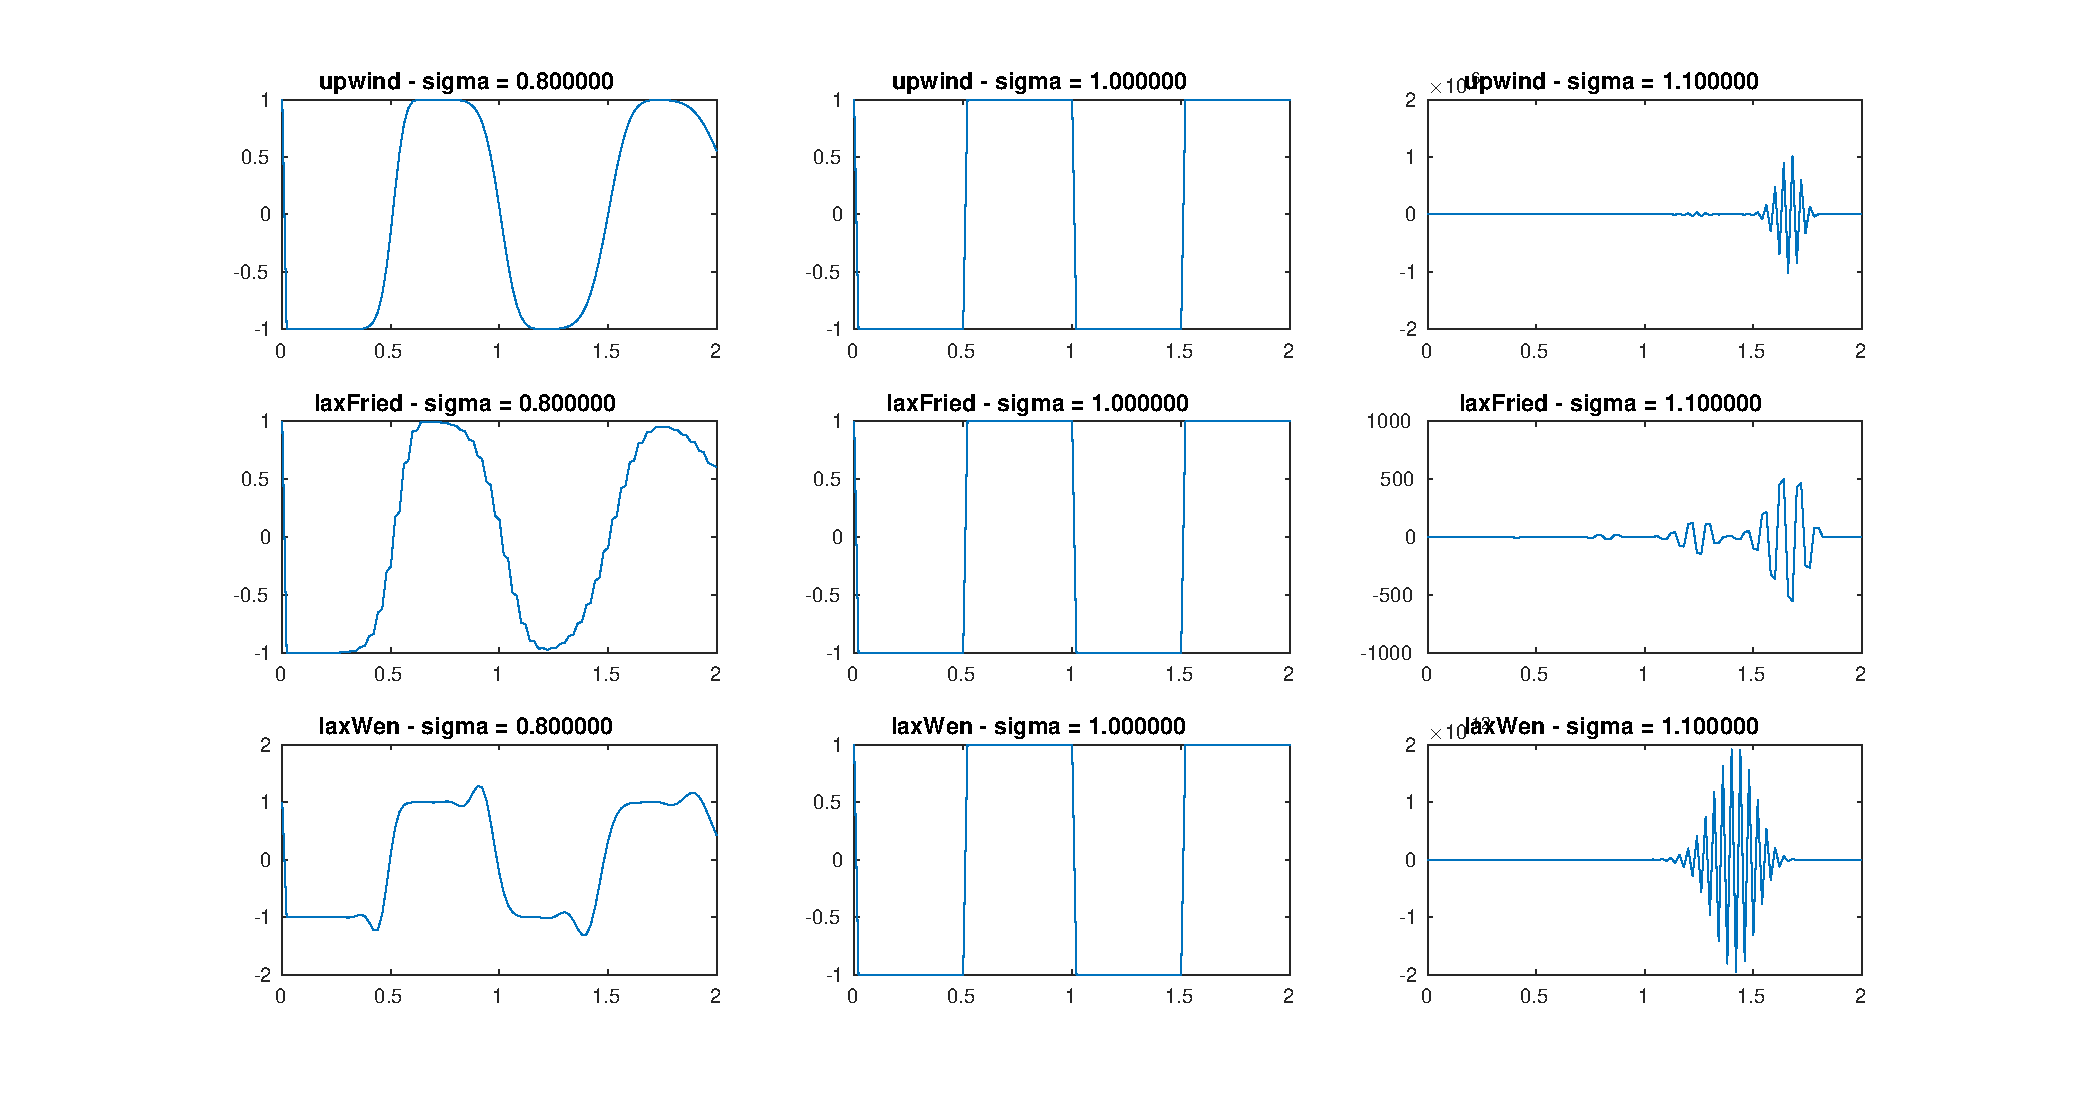
\includegraphics[scale = 0.5]{./fig1.eps}
\caption{Value of $u(x,2T)$ for the different methods}
\label{fig:1}
\end{figure}
\FloatBarrier

\subsection*{Part 2}
We are now concerned with the example 8.1 and we will try different methods to solve it.
\subsection*{a) Upwind method} 

We are first going to use the upwind method to solve the problem. The first step is to discretize the equation. The PDE is :

$$\frac{\dr T}{\dr t}+v\frac{\dr T}{\dr x}+ a(T-T_{cool})=0$$

Using forward time and backward space differences and denoting $T_{i,k} \approx T(ih_x,kh_t)$, we get :

\begin{align*}
&\frac{T_{i,k+1}-T_{i,k}}{h_t}+v\frac{T_{i,k}-T_{i-1,k}}{h_x}+a(T_{i,k}-T_{cool})=0\\
&T_{i,k+1} = (1-\frac{vh_t}{hx}-ah_t)T_{i,k}+\frac{vh_t}{h_x}T_{i-1,k}+ah_tT_{cool}
\end{align*}

Because we have an initial condition and a boundary condition for $x=0$, we problem is well posed. Figure \ref{up} presents the results for the implementation of the upwind method for the given problem.

The figure presents what is to be expected. At $x=0$, we can see the given boundary condition. We also see that the temperature propagates along the x-axis but that there are some dissipation and that the mean temperature decreases as we go along the x-axis.

\subsection*{b) Derivation of the Lax-Wendroff rule}
In this part, we are going to try to compute a Lax-Wendroff rule for the problem. The trick is to use the PDE to express the time derivatives with spacial derivatives and then use Taylor expansion. So, in this instance, we have :

$$\frac{\dr T}{\dr t}=-v\frac{\dr T}{\dr x}-a(T-T_{cool})$$

So the second order derivative, we have :
\begin{align*}
\frac{\dr^2T}{\dr t^2} &= \frac{\dr}{\dr t}( -v\frac{\dr T}{\dr x}-a(T-T_{cool}))\\
&=-v\frac{\dr}{\dr x}(\frac{\dr T}{\dr t})-a\frac{\dr T}{\dr t}\\
&=-v\frac{\dr}{\dr x}(-v\frac{\dr T}{\dr x}-a(T-T_{cool})) - a(-v\frac{\dr T}{\dr x}-a(T-T_{cool}))\\
&=v^2\frac{\dr^2 T}{\dr x^2}+2av\frac{\dr T}{\dr x}+a^2(T-T_{cool})
\end{align*}

Now we use Taylor expansion up until the second order : 
\begin{align*}
T_{i,k+1} &= T_{i,k}+h_t \frac{\dr T}{\dr t}+\frac{h_t^2}{2}\frac{\dr^2 T}{\dr t^2}\\
&=T_{i,k}+h_t(-v\frac{\dr T}{\dr x}-a(T-T_{cool}))+\frac{h_t^2}{2}(v^2\frac{\dr^2 T}{\dr x^2}+2av\frac{\dr T}{\dr x}+a^2(T-T_{cool})) 
\end{align*}

Using central differences for spatial derivatives, we get : 
$$T_{i,k+1} = c_1T_{i-1,k}+c_2T_{i,k}+c_3T_{i+1,k}+c_4$$

Where the $c_i$ are defined by : 
\begin{align*}
c_1 &= \frac{h_tv}{2h_x}+\frac{h_t^2v^2}{2h_x^2}-\frac{-avh_t^2}{2h_x}\\
c_2 &=1-ah_t+\frac{a^2h_t^2}{2}-\frac{v^2h_t^2}{h_x^2}\\
c_3 &= -\frac{vh_t}{2h_x}+\frac{v^2h_t^2}{2h^2}+\frac{avh_t^2}{2h_x}\\
c_4 &= (ah_t - \frac{a^2h_t^2}{2})T_{cool}
\end{align*}



\end{document}